\documentclass[]{article}

%opening

\usepackage{amsmath}
\usepackage{amsfonts}
\usepackage{float}
\usepackage{hyperref}
\usepackage[explicit]{titlesec}
\usepackage{xcolor}
\usepackage{graphicx}
\usepackage{indentfirst}

\title{Final Report}
\author{
	Nikolay Pavlenko\\
	\texttt{n.pavlenko@innopolis.university}
}
\begin{document}
	\maketitle
	\section{Introduction}
	After reading the paper \cite{main} I have decided not to deviate from the models that they have established for text detoxification as they demonstrated very good results against state-of-the-art methods from that time, and I do not believe myself capable of outpacing their achievements for the purpose of a single course assignment. Therefore, my final solution is the CondBERT model re-trained on a larger vocabulary, and its performance is evaluated against simple pre-trained CondBERT and paraGeDi models. \\
	
	The two primary models, paraGeDi and CondBERT, play significant roles in the task of text detoxification. paraGeDi, an extension of the GeDi model, effectively directs language models like GPT-2 to generate text on specific topics while decreasing toxicity. Conversely, CondBERT is a specialized adaptation of BERT tailored for detoxifying text. Its approach involves detecting toxic words, suggesting replacements using BERT, and employing tactics to preserve the original content. I came up with a hypothesis that aims to improve CondBERT by enlarging its dictionary with tokens from the original dataset to enhance its ability to predict text toxicity. These models present distinct methodologies for addressing text detoxification challenges. 
	\\
	\section{Data analysis}
	Before moving forward with the selection of a model for detoxification, I had to analyse the data. The original dataset is a filtered ParaNMT-detox corpus (500K sentence pairs), which contains 2 categorical columns: 
	\begin{itemize}
		\item \textbf{reference} - sentence to be detoxified
		\item \textbf{translation} - paraphrased version, supposedly less toxic
	\end{itemize}
	
	It also contains 4 numerical columns: 
	\begin{itemize}
		\item \textbf{ref\_tox} - toxicity level of reference text
		\item \textbf{trn\_tox} - toxicity level of translation text
		\item \textbf{similarity} - cosine similarity of reference and translation
		\item \textbf{lenght\_diff} - relative difference of length between reference and translation
	\end{itemize}
	
	Given the structure of the dataset, my assumption was that we have to find a model that would translate the reference into a non-toxic sentence and then we would compare the resulting translation with the existing one in the dataset. \\
	
	Investigation into the data has revealed that it has no zero values and several interesting mathematical properties:
	
	\begin{figure}[H]
		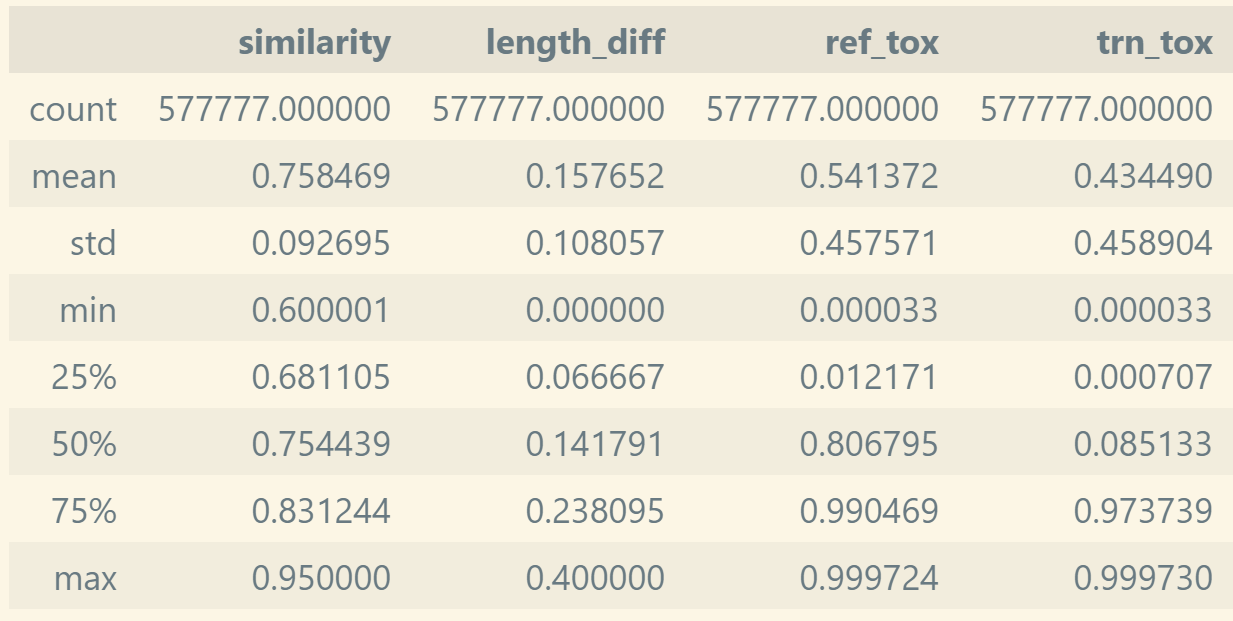
\includegraphics[scale=1]{../figures/data1.png}
		\caption{Characteristics of the original data}
	\end{figure} 
	
	I have noticed that the means of \textbf{ref\_tox} and \textbf{trn\_tox} are very similar, so it is possible that the split into toxic references and non-toxic translations does not exist in the original data. To rectify that, I create a new dataset that is used by my detoxification models. This new dataset has four features, rather than 6:
	
	\begin{itemize}
		\item \textbf{toxic} contains the \textbf{reference} if \textbf{ref\_tox} is less than \textbf{trn\_tox}, and the \textbf{translation} otherwise.
		\item \textbf{non-toxic} contains the \textbf{translation} if \textbf{ref\_tox} is less than \textbf{trn\_tox}, and the \textbf{reference} otherwise.
		\item \textbf{old\_toxicity} contains the \textbf{trn\_tox} if \textbf{ref\_tox} is less than \textbf{trn\_tox}, and the \textbf{ref\_tox} otherwise.
		\item \textbf{new\_toxicity} contains the \textbf{ref\_tox} if \textbf{ref\_tox} is less than \textbf{trn\_tox}, and the \textbf{trn\_tox} otherwise.
	\end{itemize} 
	
	The dataset above can be safely used in detoxification tasks, as it has clearly separated the toxic sentences from non-toxic. Its mathematical properties prove my point:
	
	\begin{figure}[H]
		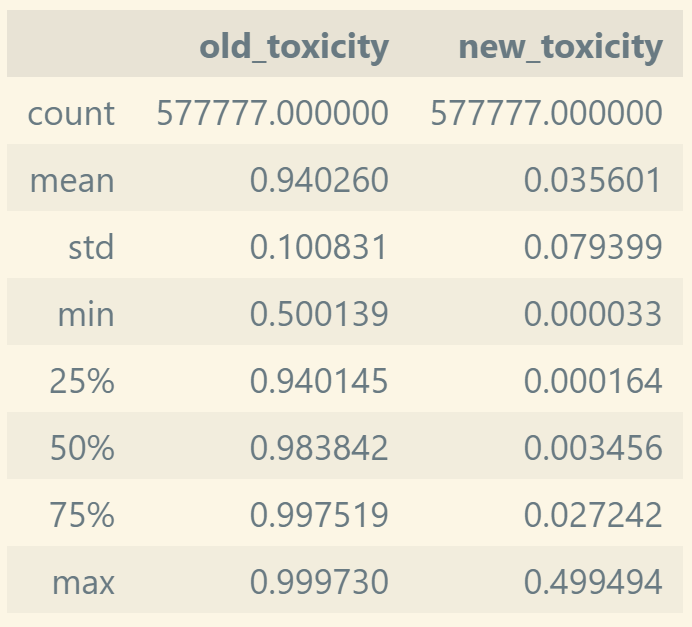
\includegraphics[scale=1]{../figures/data2.png}
		\caption{Characteristics of the modified data}
	\end{figure}
	
	\section{Model Specification}
	
	Model that is used for my final solution is CondBERT, which is a specialized adaptation of BERT, designed for the task of rewriting the text in a different style. It utilizes a series of steps to identify and replace toxic words in sentences.
	\begin{enumerate}
		\item \textbf{Toxic Word Detection}: The model detects toxic words within input sentences by fetching a toxicity score for each word from the dictionary.
		\item \textbf{Toxic Word Substitution}: It generates possible substitutes for the identified toxic words using BERT, a language model, and reranks these substitutes based on their similarity and toxicity scores.
		\item \textbf{Adaptive Threshold}: A dynamic threshold is used to determine toxic words, balancing the proportion of marked toxic words within a sentence.
		\item \textbf{Content Preservation Heuristics}: The model employs various strategies to maintain the meaning of the replaced words. It prioritizes original tokens, reorders replacements based on the similarity of their embeddings to the original words' embeddings, and penalizes tokens with positive toxicities.
		\item \textbf{Multiple Token Replacement}: It allows BERT to replace a single masked token with multiple tokens using a beam search approach and scores the sequences based on their token probabilities.
		\item \textbf{Inference Efficiency}: While considering multiple tokens can enhance accuracy, it may also increase inference time. The model aims to balance between complexity and efficiency for practical use.
		
	\end{enumerate}
	
	\section{Training Process}
	
	To make CondBERT better fit the dataset I have, I have decided to follow the training procedure proposed in \cite{main}, though slightly modified. In their training of CondBERT they use a logistic regression function to learn whether a token is toxic or not, using the pre-set vocabulary of words. Instead of creating the vocabulary from 0, in my training process I increment the already pre-trained vocab with all tokens from my dataset. This increases the knowledge model has about different toxic and non-toxic words, and allows it to find better candidates for replacement during the detoxification. \\
	
	Another necessary modification I made to ensure that the training works, was to modify the number of iterations of the logistic function from 1000 to 10000. An increase in vocabulary size also increased the complexity of logistic regression, and 1000 iterations where insufficient for it to converge. 
	
	\section{Evaluation}
	The evaluation is performed separately for pre-trained CondBERT model, for pre-trained paraGeDi model and for CondBERT model trained on the given dataset. To demonstrate differences between the models performing detoxification I made them translate the same sentences:
	
	\begin{figure}[H]
		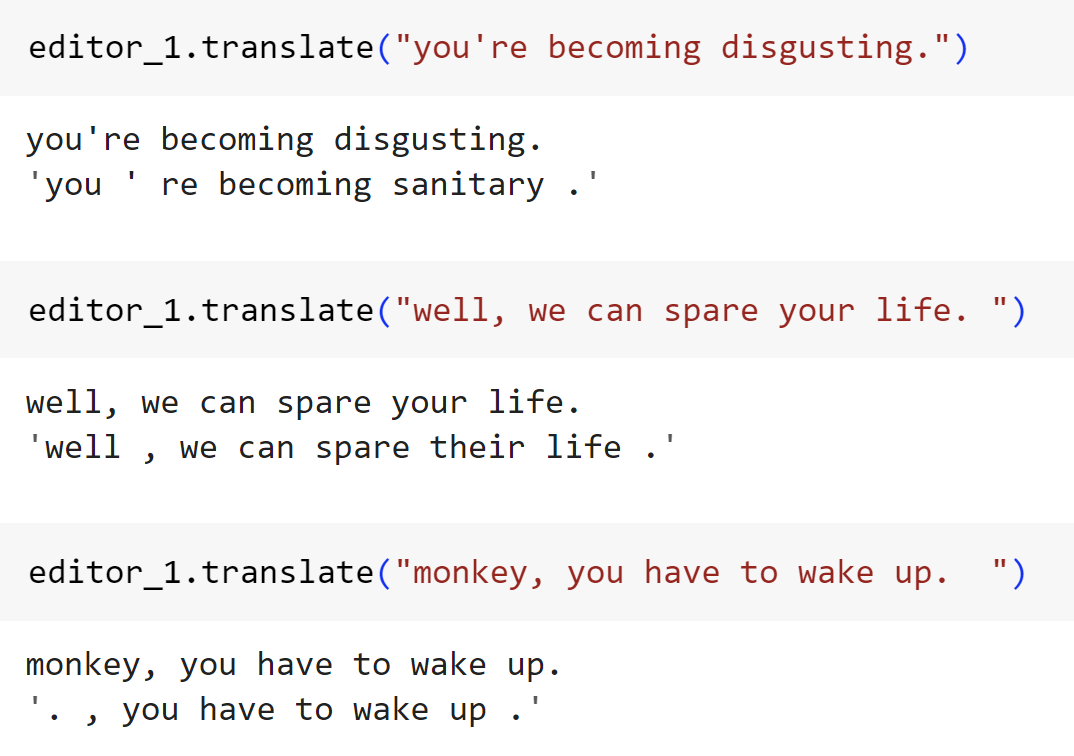
\includegraphics[scale=1]{../figures/cbtra.png}
		\caption{Translations of pre-trained CondBERT}
	\end{figure} 
	
	\begin{figure}[H]
		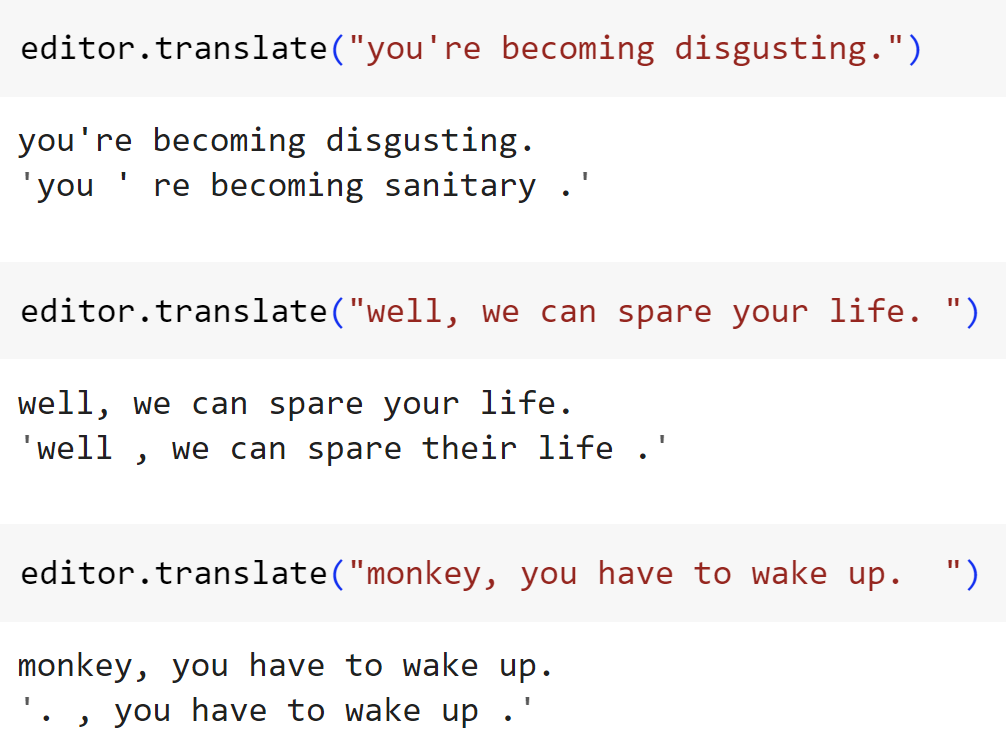
\includegraphics[scale=1]{../figures/cb2tra.png}
		\caption{Translations of fine-tuned CondBERT}
	\end{figure} 
	
	\begin{figure}[H]
		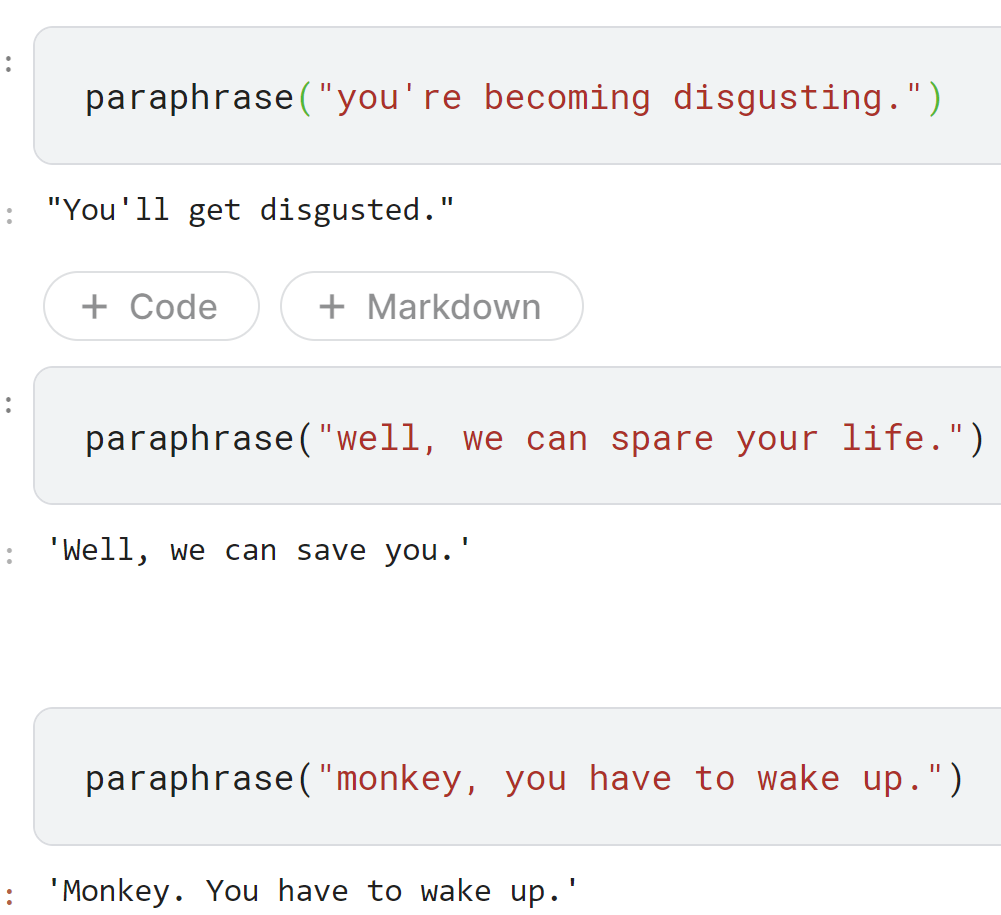
\includegraphics[scale=1]{../figures/parapa.png}
		\caption{Translations of pre-trained paraGeDi}
	\end{figure} 
	
	For further For evaluation purposes we will be using metrics from the aforementioned paper: \textbf{J}-score, \textbf{ACC}, which were implemented in the PMLDL\_Assignment1/detox/emnlp2021/metric/metric.py file. The comparison with the existing dataset will be conducted through the \textbf{ACC} metric, as we cannot afford to manually gather the data on the toxicity of reformulated sentences by the model from many different people. \\
	
	Unfortunately, calculation of the metrics as performed in that file takes an unexpectedly significant amount of time and due to time constraints their results will not be present in the current version of the report.
	
	\section{Results}
	
	The re-trained CondBERT has proven to be at least as effective at detoxification task as the pre-trained model, and considering that it has a larger vocabulary, it will perform better in general. A comparison between CondBERT and paraGeDi translations showcases that while paraGeDi is significantly better at generating human-like text due to its usage of GPT-2, it is worse at strictly identifying toxic words, as in the examples I have shown above it fails to understand that disgusting and disgusted are both not very nice words, and fails to recognize that monkey can be an insult.
	
	
	\begin{thebibliography}{99}
		\bibitem{main} Dale D. et al. Text detoxification using large pre-trained neural models //arXiv preprint arXiv:2109.08914. – 2021.
	\end{thebibliography}
	
\end{document}



